%!TEX root=masterproef.tex

\chapter{Discussie}
\label{chapter:discussie}

Dat het prototype van de generator doet wat beoogt werd kan nagegaan worden
door de gegenereerde code te inspecteren. We illustreerden dit reeds tijdens de
bespreking van de implementatie in sectie \ref{section:generation}. Hier zagen
we hoe de generator bepaalde patronen in de FOO-lang broncode omzet naar code
die inderdaad tegemoet komt aan de typische problemen die kunnen ontstaan
indien implementaties van verschillende algoritmes eenvoudig naast elkaar
geplaatst worden.

In dit hoofdstuk gaan we echter dieper in op deze vaststelling en trachten de
kwaliteit van de oplossing te quantificeren. In sectie \ref{section:setup}
introduceren we eerst de opstelling en de algoritmes die we wensen te
implementeren. Na deze situatieschets defini\"eren we in sectie
\ref{section:criteria} de evaluatecriteria en bepalen de theoretische
resultaten die we zouden verwachten gegeven de mogelijkheden tot generatie die
in eerdere hoofdstukken werden voorgesteld.

Sectie \ref{section:results} presenteert en evalueert de resultaten van de
uitvoering van de metingen.

\section{Opstelling}
\label{section:setup}

Om de generator te kunnen evalueren werd een eenvoudige opstelling gemaakt, die
toch functioneel representatief is en de mogelijkheid biedt om de
ge\"introduceerde concepten te testen.

De opstelling bestaat uit twee belangrijke luiken: een hardware/netwerk
opstelling en een selectie van detectiealgoritmes.

\subsection{Hardware en netwerk}
\label{subsection:eval-hardware}

Het DSN dat voor deze opstelling gerealiseerd werd is gebaseerd op de Zigbee
netwerkinfrastructuur en bestaat uit 3 knopen: een eindknoop, een router en een
co\"ordinator. De configuratie van de verschillende radio modules werd zo
ingesteld dat deze topologie op kleine schaal toch gerealiseerd werd. Hiertoe
werd een extra netwerk-laag in software toegevoegd. Deze laag zorgt o.a. voor
een simulatie van het feit dat elke knoop berichten van een andere knoop kan
\emph{afluisteren}. De elementaire hardware die gebruikt werd voor het
draadloze netwerk liet dit in feite niet toe. In bijlage \ref{virtual-mesh}
wordt deze virtuele netwerklaag in meer detail toegelicht.

De sensorknopen zijn niet gebaseerd op een welbepaald bestaand platform, maar
zijn samengesteld uit een \mcu en een Zigbee module. Meer specifiek werd
gebruik gemaakt van een Atmel ATMEGA1284p \citep{datasheet:atmega1284p} en een
Digi XBee 2 module \citep{manual:xbee}. Bijlage \ref{hardware-platform}
bespreekt de opbouw van de resulterende sensorknoop.

De keuze om geen standaard platform te kiezen was een duidelijke keuze. De
gekozen \mcu is een veel gebruikte architectuur en komt voor in veel
hedendaagse standaard platformen en sensorknopen, zoals bv de Atmal RZRAVEN
ontwikkelkit \citep{manual:rzraven} of het Arduino open bron electronica
platform \citep{url:arduino}.

Door gebruik te maken van elementaire componenten wordt het platform herleid
tot zijn fundamentele basis. Zo kan de generator ge\"evalueerd worden in een
context die geen voordelen nog nadelen biedt. Standaard platformen komen tevens
veelal met een eigen raamwerk voor ontwikkeling of nood aan een vorm van
besturingssysteem. Vertrekken van deze elementaire basis zorgt ervoor dat elke
toevoeging van standaardisatie van het platform of toevoeging van een hoger
niveau van abstractie op softwarevlak, eerder voordelen biedt voor de
implementatie van de generator en dit eenvoudiger maakt. Met dit platform zijn
we van mening dat er een representatieve minimale basis bestaat waar de
generator in staat voor is om code te genereren.

\subsubsection{Basis- en toepassingssoftware}

Naast de hardware en de virtuele netwerklaag, wordt verder gebruik gemaakt van
een minimale abstractielaag boven de hardware. Opnieuw met dezelfde filosofie
in gedachte, zorgt deze minimalistische tussenlaag voor een situatie waarbij de
eisen die aan het onderliggende platform gesteld worden minimaal zijn. De
functionaliteit die gebruikt worden beperkte zicht tot elementaire operaties
aangaande het netwerk:

\begin{itemize}

  \item wachten tot het netwerk beschikbaar is

  \item het opvragen van het eigen netwerkadres en dat van de hoger liggende
  knoop

  \item het verzenden van een pakket
  
  \item het ontvangen van een pakket

\end{itemize}

Om de opstelling te voorzien van een functionele toepassing, werd een
lichtsensor toegevoegd aan de knopen. De toepassing van het netwerk meet op
geregelde tijdstippen de lichtintensiteit en stuurt deze naar de co\"ordinator
van het netwerk.

\subsection{Detectiealgoritmes}
\label{subsection:eval-algorithms}

Naast de functionele toepassing, worden twee detectiealgoritmes
ge\"implementeerd. Het betreft een implementatie van het elementaire
\emph{heartbeat} principe en een algoritme dat op basis van observaties in het
netwerk een waardering opbouwt betreffende de betrouwbaarheid van andere knopen.

Beide algoritmes werden in FOO-lang beschreven en zijn opgenomen in bijlage
\ref{appendix:demo-code}.

\subsubsection{\emph{Heartbeat}}

Hierbij zenden knopen op gestelde tijdstippen een
pakket uit. Andere knopen kunnen deze sequentie van berichten opvolgen en bij
het ontbreken van zulke berichten de beschikbaarheid van een knoop in vraag
stellen. Ofschoon minimalistisch van aard, is het structureel toch
representatief voor eenvoudige detectiealgoritmes die gegevens uitsturen,
binnenkomende berichten verwerken en een minimale staat van andere knopen
bijhouden en aggregeren tot een beslissing.

De voorgestelde implementatie gebruikt ook een SHA1 hash \citep{rfc:3174} om
een digitale handtekening toe te voegen aan het bericht. Zonder de
betrouwbaarheid van deze aanpak te willen in vraagstellen, staat het gebruik
ervan eerder in functie van het aantonen dat cryptografische en externe
functionaliteit kan gebruikt worden.

\subsubsection{Reputatie}

Het tweede algoritme is een implementatie van het principe dat voorgesteld werd
in sectie \ref{subsection:reputation}. Door op te volgen of een hoger liggende
knoop in het netwerk, berichten effectief verder doorheen het netwerk stuurt,
wordt statistisch bepaald of deze knoop betrouwbaar is of niet.

Dit algoritme voegt nog enkele complexiteiten toe en vraagt dat arbitraire
berekeningen kunnen uitgevoerd worden en dat de resultaten er van kunnen
ge\"interpreteerd worden. Ook wordt hier de complexiteit toegevoegd waarbij
omgegaan moet worden met volledige netwerkpakketten.

\subsubsection{Configuratie}

De configuratie van beide algoritmes is natuurlijk van belang. Een configuratie
die niet resulteert in een concurrentie tussen beide algoritmes zal weinig tot
geen optimalisatie laten optekenen.

De mogelijkheden tot configuratie liggen in de tijden tussen twee uitvoeringen
van een functioneel aspect van het algoritme. In beide gevallen gaat dit om een
tussentijd vooraleer het algoritme zelf een bericht uitstuurt en de tussentijd
waarop een evaluatie van de geaggregeerde informatie gebeurt. Het eerste aspect
bepaalt de synchroniciteit van het uitsturen van berichten en of er
mogelijkheid is tot samennemen van berichten om zo het draadloze netwerk te
ontlasten. Het punt van evaluatie bepaalt of het overlopen van alle gekende
knopen voor beide algoritmes tegelijk kan gebeuren of niet.

Om een situatie af te dwingen waar de voordelen van de oplossing zich zouden
moeten manifesteren, werd geopteerd voor volgende configuratie:

\begin{itemize}

  \item de tijd tussen twee opeenvolgende \emph{heartbeats}: 3s

  \item de tijd tussen twee opeenvolgende verzendingen van informatie
  betreffende reputatie: 7,5s

  \item in beide gevallen: de tijd tussen twee opeenvolgende evaluaties: 5s

\end{itemize}

\section{Evaluatiecriteria}
\label{section:criteria}

De doelstelling om de impact van de introductie van een IDS in een DSN te
verlagen is de basis voor de evaluatiecriteria. Bij het uitdiepen van de
probleemstelling in hoofdstuk \ref{chapter:probleemstelling} werd het
ontwikkelingsproces gevolg van de hardware en het onderzoek tot de software en
de uitbating. Hieruit distilleren we de volgende functionele en
niet-functionele criteria.

\subsection{Functionele criteria}

Elk van de ontwikkelde componenten in deze masterproef dient een functioneel
doel:

\begin{description}

  \item[Expressiviteit] Vanuit functioneel oogpunt moet de voorgestelde taal in
  staat zijn om de beschrijving van een representatieve selectie van
  detectiealgoritmes mogelijk te maken. Concreet moet aan de hand van FOO-lang
  het mogelijk zijn om de voorgestelde algoritmes correct en zonder
  noodzakelijke omwegen te implementeren.

  \item[Automatiseerbaarheid] De code generator moet het mogelijk maken om op
  een volledig geautomatiseerde manier een IDS toe te voegen aan een te
  integreren toepassing.

\end{description}

\subsection{Niet-functionele criteria}

De niet-functionele criteria hebben betrekking op de impact van het IDS op de
middelen van de sensorknopen. In essentie komt dit neer op het energieverbruik.
We vertalen dit concept in deze context naar twee overeenkomstige en direct
be\"invloedende factoren: het gebruik van de draadloze radio en de tijd om
\'e\'en cyclus van de \emph{event-loop} te doorlopen. Het gebruik van de radio
wordt verder opgesplitst in het aantal verzonden pakketten en de hoeveelheid
aan gegevens die worden verstuurd.

\begin{description}
  
  \item[Aantal verzonden netwerkpakketten] Het aantal verzonden pakketten
  bepaalt hoe dikwijls de radio effectief moet zenden. Dit is typisch het
  kostelijkste wat betreft energieverbruik. Het verminderen van het aantal
  pakketten heeft dus een rechtstreekse relatie met het energieverbruik.

  \item[Aantal verzonden bytes] Het opvolgen van het aantal bytes die effectief
  verstuurd worden is van belang om in te schatten dat de eventuele winst door
  een afname van het aantal verzonden pakketten niet gecompenseerd wordt door
  een toename in het aantal effectief verzonden bytes.

  \item[Lengte event-loop] De doorlooptijd van \'e\'en cyclus van de
  \emph{event-loop} bepaalt hoe lang de \mcu effectief actief is. Typisch wordt
  op het einde van elke cyclus een periode ingelast van niet-activiteit. De
  cyclus plus de rustperiode zijn typisch een constante, waardoor het aandeel
  van de cyclus een relatieve impact heeft op het energieverbruik.
  
\end{description}

Naast deze drie energie-gebonden criteria kunnen we nog een vierde cirterium in
beschouwing nemen, nl. de grootte van de resulterende code die naast de
applicatiecode moet ge\"installeerd worden op de sensorknoop.

Dit is echter een noodzakelijk kwaad. Dat de introductie van een IDS een impact
zal hebben op dit vlak is evident. We moeten dus opnieuw een vergelijking maken
met de manuele situatie en kijken hoeveel de gegenereerde code eventueel groter
is.

\subsection{Theoretische evaluatie}

Gegeven de doelstellingen en de configuratie is het mogelijk een voorspelling
te doen van bepaalde van de niet-functionele criteria. Wanneer we een periode
van 90 seconden in beschouwing nemen en de de activiteiten van de algoritmes
hierbinnen uitzetten, dan kunnen we het aantal verzonden netwerkpakketten
berekenen.

De toepassing verstuurt om de 5 seconden een meting van de lichtsensor. Dit
resulteert 18 netwerkpakketten. Het \emph{heartbeat} algoritme verstuurt elke 3
seconden een pakket. Dit resulteert in 30 pakketten. Het reputatie-gebaseerde
algoritme verstuurt informatie om de 7,5 seconde of wel nog eens 12 pakketten.

Over een periode van 90 seconden verwachten we dus dat er 18 + 30 + 12 = 60
pakketten verzonden zullen worden.

Indien we aannemen dat de generator effectief er voor zorgt dat berichten die
dicht bij elkaar verzonden worden, gebundeld worden in \'e\'en pakket, dan zal
zich op gemeenschappelijk veelvouden van 3 en 7,5 deze situatie aanbieden.
Concreet zal dit zijn op de veelvouden van 15, ofwel in op 6 ogenblikken.

We zouden bij de gegenereerde code dus een reductie van 6 pakketten moeten
kunnen optekenen over een zelfde periode.

\section{Evaluatie van de functionele criteria}

De twee functionele criteria focussen elk op \'e\'en van de twee grote
componenten die binnen de scope van deze masterproef vallen: FOO-lang en de
code generator.

\subsection{Een derde algoritme}

Om FOO-lang zelf te evalueren werd een derde algoritme beschreven. Hierbij werd
nagegaan welke uitbreidingen of aanpassingen aan FOO-lang nodig waren om dit
derde algoritme op een gelijkwaardige manier te kunnen beschrijven.

Het algoritme in kwestie was het co\"operatieve algoritme beschreven in sectie
\ref{subsubsection:cooperation-algorithm}. De experimentele beschrijving is
terug te vinden in bijlage \ref{lst:cooperation.foo}.

De conclusie van deze oefening is dat er nog enkele typische constructies
ontbreken aan FOO-lang, wat in de lijn van de verwachting lag, maar dat de
meeste tekorten eerder te wijten zijn aan de minimale implementatie van de
voorzien mogelijkheden.

De concepten van de taal blijven overeind en de aanpassingen zijn meestal
uitbreidingen van bestaande constructies met bijkomende mogelijkheden of een
andere scope.

\subsection{De generator}

De generator biedt met een API en een CLI toepassing een uitermate flexibele
interface naar de buitenwereld toe. Op deze manier is een integratie in een
ontwikkelingsproces zeer vlot realiseerbaar. Bij wijze van illustratie is elke
test die uitgevoerd werd voor deze masterproef zeer eenvoudig op te starten met
\'e\'en enkele oproep van een door een \emph{Makefile} georganiseerd
generatie-, compilatie- en installatieproces.

Een ander aspect dat van belang is in de context van de generator is de
uitbreidbaarheid. Bij het prototype is uitgegaan van een minimalistische
situatie met een \emph{event-loop}. Indien men bv. ondersteuning zou willen
inbouwen voor Contiki of een ander besturingssysteem dient hiervoor een nieuwe
Python module geschreven te worden die mee de vertaling dient te doen aan de
hand van model transformaties.

Dit vraagt zonder meer werk en een juiste inschatting van de hoeveelheid is
zeer platform-afhankelijk. Hier kan slechts een indicatieve richting aangegeven
worden op basis van de ervaring bij het ontwikkelen van de software voor de
evaluatie. Het schrijven van een manuele versie op basis van enkele losse
modules geeft een goed beeld van hoe de integratie dient te gebeuren. Mits een
korte analyse van deze manuele code en een koppeling naar de typische concepten
die FOO-lib aanbiedt, kan de creatie van zo'n module vlot gebeuren. Dit is
tevens een \'e\'enmalige investering die bij elke volgende generatie zich zelf
snel terug betaalt.

\section{Resultaten en evaluatie van niet-functionele criteria}
\label{section:results}

Voor deze evaluatie werd zowel een volledig manuele implementatie gemaakt als
een gegenereerde. Zowel de manuele implementatie als de gegenereerde
implementatie werd opgebouwd met een zelfde programmeerstijl en maakt geen
gebruik van enige voorkennis omtrent de algoritmes. De manuele implementatie
bestaat uit een basisapplicatie en twee modules voor de algoritmes.

Deze modules werden vervolgens sequentieel ingevoegd in de basisapplicatie,
zoals dit het geval zou zijn indien men bestaande implementaties kon
hergebruiken. Dit resulteert structureel in twee oproepen naar de modules
vanuit de event-loop en twee oproepen wanneer een bericht ontvangen wordt.

\subsection{Metingen}

Het tellen van het aantal verzonden pakketten en bytes werd toegevoegd aan de
minimale abstractielaag en is dus een constante bijkomende belasting in alle
gevallen.

Om de doorlooptijd van de event-loop te meten, werd het aantal cycli dat de
event-loop doorliep gemeten gedurende een interval van 15 seconden. Hieruit
werd de doorlooptijd van \'e\'en cyclus berekend. De reden van deze opstelling
is het feit dat de \mcu slechts een kloksnelheid heeft van 8MHz. Hiermee is het
mogelijk om aan de hand van \emph{interrupts} een virtuele klok te bouwen die
milliseconden kan meten. Een grotere precisie, bv. microseconden, zal een te
groot deel van de rekentijd van de \mcu vragen, waardoor de toepassing niet
genoeg tijd meer krijgt om effectief te werken.

Naast deze aanpak werd ook gebruik gemaakt van een \emph{logic analyser}. Door
aan het begin van een oproep naar een module van een detectiealgoritme hoog
signaal uit te sturen op \'e\'en van de uitvoer pinnen van de \mcu en dit op
het einde van de oproep opnieuw laag te brengen, kunnen we deze verschillen
extern meten. Dit laat toe om zelfs sub-microseconde verschillen te meten.

Met de beschikbare middelen was het niet mogelijk om een totaalbeeld te vormen
over een periode van 90 seconden, maar de meting liet wel toe om de situatie
waarbij in een cyclus van de event-loop geen enkele actie ondernomen werd door
het IDS, in kaart te brengen. Deze situatie toont de minimale, constante extra
belasting die het IDS met zich meebrengt.

\subsection{Resultaten}

Tabellen \ref{tbl:manual} en \ref{tbl:generated} tonen de ruwe metingen voor
respectievelijk de manuele en de gegenereerde implementatie. De verschillende
niet-functionele criteria worden voor de verschillende configuraties uitgezet.
De eerste situatie is die van de naakte applicatie, zonder enige vorm van IDS.
Dit is de referentie voor de andere configuraties. Daarnaast zijn drie
configuraties geplaatst: \'e\'en met alleen het \emph{heartbeat} algoritme
toegevoegd, \'e\'en met alle het reputatie-algoritme toegevoegd en \'e\'en met
beide algoritmes.

Naast de ruwe meetwaarde is tevens een procentuele vergelijking met de
referentie opgenomen om de impact beter te quantificeren.

\begin{table}[H]
  \centering
  \begin{tabular}{l|r|rr|rr|rr}
  \hline
      & zonder & \multicolumn{2}{c|}{heartbeat} & \multicolumn{2}{c|}{reputatie} & \multicolumn{2}{c}{beide} \\
  \hline
  \hline

aantal frames         &    20    &    51    & 255\% &    32    & 160\% &    63    & 315\% \\
aantal bytes          &   476    &  1933    & 406\% &   860    & 181\% &  2317    & 487\% \\
gemiddeld bytes/frame &    23.80 &    37.90 & 159\% &    26.88 & 113\% &    36.78 & 155\% \\
doorlooptijd ($\mu$s) &    48    &    94    & 196\% &    88    & 183\% &   149    & 310\% \\
grootte (bytes)       & 10500    & 15530    & 148\% & 13306    & 127\% & 18334    & 175\% \\

  \hline
  \end{tabular}
  \caption{Resultaten voor de manuele implementatie}
  \label{tbl:manual}
\end{table}

Wanneer we de referentie bij de manuele implementatie bekijken zien we dat er
inderdaad zoals verwacht (ongeveer) 19 pakketten verstuurd zijn.\footnote{Het
bijkomende pakket is toe te schrijven aan een bijkomend pakket dat tijdens het
initialiseren van het virtuele netwerk gebruikt wordt door de eindknoop om de
hoger liggende knoop te vinden.} Het gemiddeld aantal bytes per frame is
(ongeveer) 24. Een lichtmeting bestaat uit 2 bytes. Daarnaast worden er 6 extra
bytes gebruikt door de implementatie van het virtuele netwerk. Het Zigbee
pakketformaat voegt nog eens 16 bytes toe \citep{alliance2012zigbee}. De totale
som, 2 + 6 + 16 is inderdaad 24\footnote{De ogenschijnlijk fout op de waarde is
opnieuw toe te schrijven aan het initi\"ele extra pakket. Dit is slechts 4
bytes groot, heeft geen bijkomende adresinformatie van het virtuele netwerk en
heeft verder alleen nog 16 bijkomende bytes van het Zigbee protocol. Zo komt
het op 20 bytes. Opgeteld bij 19 $\times$ 24 = 456 geeft dat inderdaad 476.}.

Door de introductie van het IDS stijgen deze waarden natuurlijk. We berekenden
reeds dat de introductie van een \emph{heartbeat} een bijkomende 30 pakketten
betekent en dat voor de communicatie voor het uitwisselen van
reputatie-informatie er 12 extra pakketten nodig zijn. We zien deze getallen
nagenoeg exact terugkomen in de meeteresultaten: In het geval van het
\emph{heartbeat} algoritme is er \'e\'en pakket meer verzonden. Dit was te
wijten aan een tweede initialisatie-pakket voor het opzetten van het virtuele
netwerk.

We merken verder op dat de combinatie van de twee algoritmes letterlijk een
sommatie is van de individuele impact, wat logisch is en de veronderstelling
bevestigt. In het geval van de doorlooptijd ligt deze zelfs nog iets hoger. In
plaats van 48 + 46 + 40 = 134 $\mu$s is de doorlooptijd zelfs 149 $\mu$s.

Tot slot zien we dat de manuele introductie van het IDS een vergroting van de
te installeren code van 75\% betekent. In absolute cijfers een kleine 8
kilobyte (KB).

\subsubsection{Gegenereerde code}

Tabel \ref{tbl:generated} toont exact dezelfde gegevens, maar dan voor de
gegenereerde code.

\begin{table}[H]
  \centering
  \begin{tabular}{l|r|rr|rr|rr}
  \hline
      & zonder & \multicolumn{2}{c|}{heartbeat} & \multicolumn{2}{c|}{reputatie} & \multicolumn{2}{c}{beide} \\
  \hline
  \hline
  
aantal frames	        &    20	   &    49	  & 245\%	&    32	   & 160\% &    55	  & 275\% \\
aantal bytes          &   476	   &  1897	  & 399\%	&   884	   & 186\% &  2161	  & 454\% \\
gemiddeld bytes/frame	&    23.80 &  	38.71	& 163\%	&    27.63 & 116\% &    39.29	& 165\% \\
doorlooptijd ($\mu$s) &    48    &   121	  & 252\%	&   121	   & 252\% &   138	  & 288\% \\
grootte (bytes)       &	10496	   & 18352	  & 175\%	& 16376	   & 156\% & 20998	  & 200\% \\

  \hline
  \end{tabular}
  \caption{Resultaten voor de gegenereerde implementatie}
  \label{tbl:generated}
\end{table}

Hier merken op dat de gegenereerde referentie-implementatie nagenoeg perfect
overeenkomt met de manuele referentie-implementatie\footnote{De vier bytes
verschil zijn vermoedelijk te wijten aan twee bijkomende ongebruikte
functiedeclaraties in de manuele code. Dit werd omwille van het marginale
verschil niet verder onderzocht.}.

De zelfde getallen als bij de manuele implementatie zien we terugkomen voor het
aantal verzonden pakketten\footnote{Bij het \emph{heartbeat} algoritme werd er
geen extra pakket bij intialisering verstuurd en werd 1 pakket net niet meer
meegeteld op het einde van de 90 seconden.}

Een eerste verschil merken we echter op bij het aantal pakketten in het geval
dat beide algoritmes actief zijn. In theorie verwachtten we hier 6 pakketten
minder. Het verschil is 8. Dit is te wijten aan een extra initialiseringspakket
bij de manuele versie en een opnieuw een pakket dat net niet meegeteld werd.

Met een lengte van 20 bytes, voegt een digitale handtekening op basis van SHA1
natuurlijk bytes toe aan het gemiddelde. Ook een pakket met informatie over de
reputatie van de verschillende knopen is groter dan een lichtmeting. We moeten
hier zelfs opmerken dat het algoritme voor het verzenden van
reputatieinformatie zelf geen bundeling doet van deze informtie en dat in de
FOO-lang beschrijving er feitelijk een bericht wordt verstuurd voor elke knoop
apart. Dankzij het aggregerende karakter van de onderliggende implementatie,
zullen al deze berichten samen verstuurd worden.

Ook bij het totaal aantal verstuurde bytes zien we dat het samennemen van
pakketten een winst oplevert. Een gewone optelling van de afzonderlijke
hoeveelheden levert een totaal op van 476 + 1421 + 408 = 2305, want 144 bytes
meer is dan de gemeten waarde.

De doorlooptijd van \'e\'en cyclus van de \emph{event-loop} vraagt per
toevoeging van een algoritme ongeveer 73$\mu$s. Bij een implementatie met de
twee algoritmes is dit slechts 90 in totaal. We zien hier dat een groot deel
van de bijkomende verwerking van een algoritme toe te schrijven is aan de
softwarebibliotheek. Door deze kost te spreiden over meerdere algoritmes komt
deze investering tot uiting. Een zelfde situatie doet zich voor bij de grootte
van de te installeren code.

\subsubsection{Vergelijking}

De belangrijkste vraag die we willen beantwoorden is hoe dat de gegenereerde
code zich verhoudt tot de manuele code. Tabel \ref{tbl:comparison} vergelijkt
de eerdere resultaten door een verschil te maken tussen de twee situaties en
door een relatieve vergelijking van de configuratie met beide algoritmes.

\begin{table}[H]
  \centering
  \begin{tabular}{l|r|rrrr}
  \hline
  & zonder & heartbeat & reputatie & beide & verschil\\
  \hline
  \hline

paketten               &  0    &   -2    &    0    &   -8    & \cellcolor{green!25} 87.30\% \\
bytes                  &  0    &  -36    &   24    & -156    & \cellcolor{green!25} 93.27\% \\
gemiddeld bytes/pakket &  0.00 &    0.81 &    0.75 &    2.51 & \cellcolor{red!25}  106.83\% \\
doorlooptijd ($\mu$s)  &  0    &   27    &   33    &  -11    & \cellcolor{green!25} 92.62\% \\
grootte (bytes)        & -4    & 2822    & 3070    & 2664    & \cellcolor{red!25}  114.53\% \\

  \hline
  \end{tabular}
  \caption{Vergelijking van de manuele en gegenereerde resultaten}
  \label{tbl:comparison}
\end{table}

De resultaten bevestigen de veronderstellingen over de hele lijn: dankzij het
samennemen van pakketten kan een winst van ongeveer 10\% opgetekend worden met
betrekking tot het gebruik van de draadloze radio. Ook de doorlooptijd van een
cyclus van de event-loop vertoont een optimalisatie in die grootorde. Het feit
dat daardoor het gemiddelde aantal bytes per pakket stijgt is ook volgens
verwachting en met een stijging van ongeveer 7\% is dit zeker geen slechte
verhouding.

Ook de stijging van de grootte van de te installeren code is logisch en is met
ongeveer 15\% zeker niet onoverkomelijk. In dit geval is de absolute waarde
misschien van grotere betekenis. De introductie van het generatieraamwerk en de
bijhorende softwarebibliotheek vraagt ruwweg 3KB extra en die grootte neemt
relatief af met het aantal algoritmes die toegevoegd worden.

\subsubsection{Minimale extra verwerkingstijd}

Tot slot bekijken we nog een meting op het niveau van \'e\'en enkele cyclus van
de event-loop. Figuur \ref{fig:logic-analyser-manual} toont het verloop van de
spanning op een uitvoerpin van de \mcu. De spanning op deze pin wordt aangelegd
en weggenomen door een instructie net voor en net na het oproepen van \'e\'en
van de detectiemodules. In het geval van de manuele implementatie gebeurt dit
tweemaal per cyclus.

\begin{figure}[ht]
  \centering
  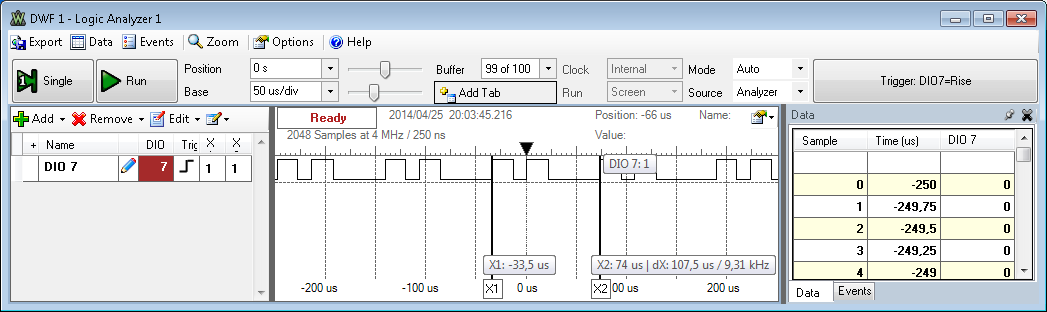
\includegraphics[width=\linewidth]{../src/demo/idle-event-loop-both-manual.png}
  \caption{Minimale activiteit in \'e\'en cyclus van de event-loop (manueel)}
  \label{fig:logic-analyser-manual}
\end{figure}

\vspace{-4mm}

In de figuur zien we deze twee ogenblikken duidelijk naar voor komen. Wanneer
we de doorlooptijd meten van \'e\'en cyclus zien we dat deze rond de 107$\mu$s
ligt. Uit tabel \ref{tbl:manual} weten we dat de gemiddelde doorlooptijd
zonder IDS 48$\mu$s bedraagt. Hieruit concluderen we dat, in de manuele
situatie, het toevoegen van een IDS een minimale extra verwerkingstijd met zich
meebrengt van 59$\mu$s of ongeveer 120\%.

Figuur \ref{fig:logic-analyser-generated} toont dezelfde situatie als voorheen,
maar nu voor de gegenereerde code. Hier zien we dat er slechts \'e\'en plateau
gevormd wordt. De verwerking van beide algoritmes is in deze situatie gebundeld
in de verwerking door het generatieraamwerk.

\begin{figure}[ht]
  \centering
  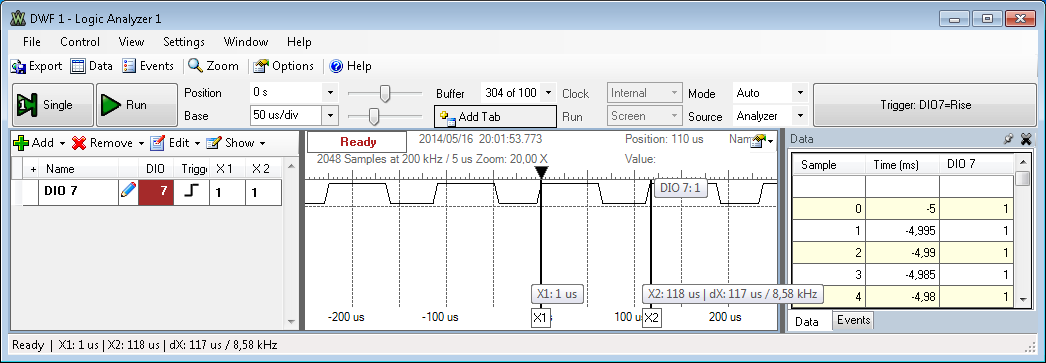
\includegraphics[width=\linewidth]{../src/demo/idle-event-loop-both-generated.png}
  \caption{Minimale activiteit in \'e\'en cyclus van de event-loop (gegenereerd)}
  \label{fig:logic-analyser-generated}
\end{figure}

\vspace{-4mm}

In het geval van de gegenereerde code, zien we dat de doorlooptijd van \'e\'en
cyclus van de event-loop zonder speciale activiteit ongeveer 117$\mu$s in
beslag neemt. Dit is 10$\mu$s meer dan bij de manuele implementatie. De
minimale extra verwerkingstijd komt zo op 69$\mu$s of 143\%.

\vspace{-4mm}

\section{Afsluitende bedenking}

Het is gevaarlijk om een evaluatie van een taal en code generator te doen aan
de hand van metingen. De cijfers gepresenteerd in dit hoofdstuk zijn
grotendeels afhankelijk van de beschreven algoritmes, de configuratie, even als
de feitelijke functionele toepassing. De enige manier waarop deze resultaten
mogen ge\"interpreteerd worden is als een vage bevestiging van wat
logischerwijs reeds kon ingeschat worden, nl. dat men door code beter te
organiseren winst kan boeken.
